\chapter{Návrh}

V kapitole \emph{návrh} postupně projdeme jednotlivé součásti a výsledného systému. Nejprve se budeme zabývat formalizací způsobu specifikace pravidel správného návrhu software.

Část druhá je věnována rozboru navrhované architektury systému. Systém je postupně dekomponován shora dolů. Hlavní funkční bloky jsou postupně dekomponovány na komponenty, jejichž realizace je triviální. Je navrhováno rozdělení systému na jádro (core) a moduly, které budou poskytovat konkrétní funkčionalitu.

Další části se věnují postupně návrhu vstupního rozhraní, výstupního rozhraní a způsobu integrace jádra do různých prostředí.

Poslední část je věnována návrhu konkrétních technologií, v nichž bude výsledný systém realizován.

\section{Návrh způsobu specifikace pravidel}

Abychom mohli specifikovat pravidla, musíme nejprve definovat strukturu, nad kterou budou tato pravidla platit. V~tomto textu formalizujeme model programu pomocí teorie grafů. Nad grafem je potom možné specifikovat pravidla, která musí vstupní projekt splňovat.

\subsection{Formalizace modelu programu pomocí grafu}
\label{design-graph_formalization}

Analyzovaný softwarový projekt abstrahujeme jako orientovaný multigraf rozšířený o~zobrazení množiny uzlů do množiny typů\footnote{Pod pojmem typ zde rozumíme jakékoliv označení, které specifikuje o~jaký objekt se jedná, nikoliv datový typ. Může se jednat o vrchol typu třída, metoda, příkaz nebo třeba celý zdrojový soubor, budeme-li analyzovat vztahy mezi kompilačními jednotkami.} a zobrazení hran do množiny jejich klasifikátorů (označení typu vztahu mezi uzly). Dále přidáme ke každému vrcholu zobrazení, které mu přiřadí jméno (řetězec). Získáme tak následující definici pojmu \emph{grafový model programu}:

\begin{definition}
\textbf{Grafovým modelem projektu} nazveme strukturu
\begin{displaymath}
  G = \langle V, E, \rho, K, C, N, \mathit{Kind}, \mathit{Classifier}, \mathit{Name}\rangle
  \label{extended_multigraph}
\end{displaymath}
v~níž platí:
\begin{itemize}
\item $V$ je množina elementů (v~našem případě části kódu)
\item $E$ je množina hran (v~našem případě vztahy mezi částmi kódu - např. volání funkce, dědičnost)
\item $V \cap E = \emptyset$
\item $\rho: E \mapsto V \times V$ je zobrazení množiny hran do množiny uspořádaných dvojic vrcholů (incidence)
\item $K$ je libovolná množina označení typů vrcholů,
\item $C$ je množina klasifikátorů hran,
\item $N$ je množina jmen (řetězců)
\item $\mathit{Kind}: V \mapsto K$ je zobrazení, které přiřadí každému vrcholu jeho typ,
\item $\mathit{Classifier}: E \mapsto C$ je zobrazení, které přiřadí každé hraně její klasifikátor (zda se jedná o~method call, dědičnost, apod.)
\item $\mathit{Name}: V \mapsto N$ je zobrazení, které přiřadí vrcholu jeho jméno (např. jméno třídy, jméno metody)
\end{itemize}
\end{definition}

Ukázka formalizace zdrojového kódu pomocí grafu je na obrázku \ref{design-graph_example}. V~uvedeném příkladě můžeme strukturu $G$ namapovat následujícím způsobem:

\begin{figure}[h!]
  \centering
  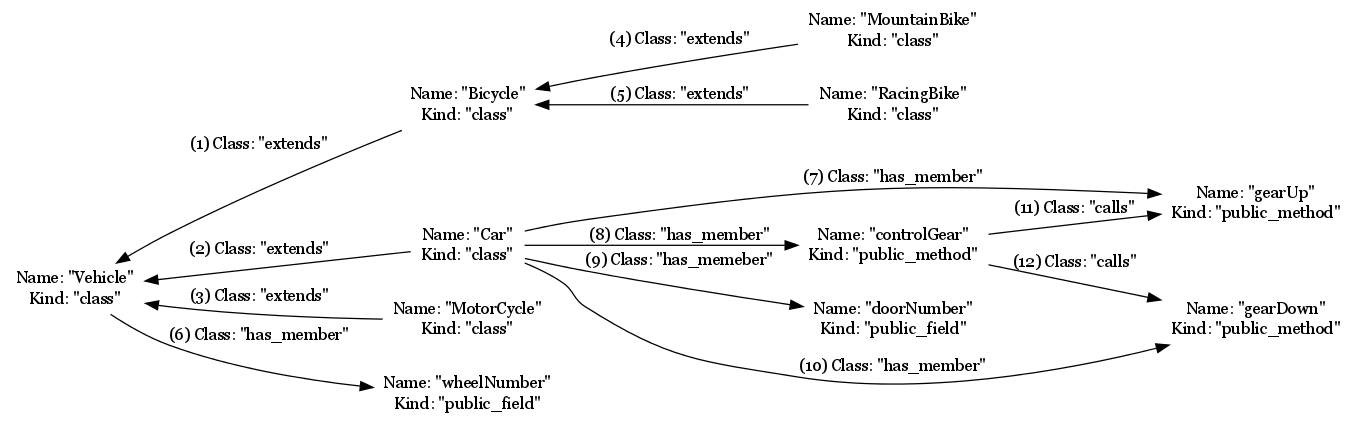
\includegraphics[width=1.0\textwidth]{./graphs/graph_example.png}
  \caption{Příklad formalizace hierarchie tříd jako grafu.\label{design-graph_example}}
\end{figure}
Množinu vrcholů můžeme ztotožnit s~množinou názvů elementů (v~našem případě třídy, pole, metody)\footnote{V konečném důsledku bude tato množina představována konkrétními elementy tak, jak se nalézají ve zdrojovém kódu.}.
\begin{align*}
  V = &\{ \\
  &``Vehicle", ``Car", ``MotorCycle", ``Bicycle", ``MountainBike", ``RacingBike", \\
  &``wheelNumber", ``doorNumber", \\
  &``controlGear", ``gearUp", ``gearDown" \\
  &\}
\end{align*}
Abychom mohli demonstrovat množinu hran, bylo provedeno očíslování. Hranu zde identifikujeme číslem. V~počítačové reprezentaci se může jednat o~konkrétní objekt (resp. referenci na něj) uložený v~poli. Zvolený identifikátor hrany nemá vliv na prováděnou analýzu, musí pouze zajistit jednoznačnou identifikaci hrany. Množinu hran zde v~textu reprezentujeme prostým výčtem čísel\footnote{V programu bude potom hrana reprezentována konkrétním objektem případně rozšířeným o~vhodný jedinečný identifikátor.}:

\begin{displaymath}
  E = \{1, 2, 3, 4, 5, 6, 7, 8, 9, 10, 11, 12\}
\end{displaymath}
Zobrazení $\rho$, které představuje přiřazení jednotlivých hran dvojicím uzlů, můžeme formálně zapsat jako následující množinu\footnote{Zobrazení je binární relace. Proto jej můžeme reprezentovat jako množinu uspořádaných dvojic.}:
\begin{align*}
  \rho = &\{ \\
  &(1, (``Bicycle", ``Vehicle")), \\
  &(2, (``Car", ``Vehicle")), \\
  &(3, (``MotorCycle", ``Vehicle")), \\
  &(4, (``MountainBike", ``Bicycle")), \\
  &(5, (``RacingBike", ``Bicycle")), \\
  &(6, (``Vehicle", ``wheelNumber")), \\
  &(7, (``Car", ``gearUp")), \\
  &(8, (``Car", ``controlGear")), \\
  &(9, (``Car", ``doorNumber")), \\
  &(10, (``Car", ``gearDown")), \\
  &(11, (``controlGear", ``gearUp")), \\
  &(12, (``controlGear", ``gearDown")) \\
  &\}
\end{align*}
Zbývají nám množina typů $K$,
\begin{align*}
  K = \{ ``class", ``public\_field", ``public\_method" \}
\end{align*}
množina klasifikátorů hran $C$,
\begin{align*}
  C = \{ ``extends", ``has\_member", ``calls" \}
\end{align*}
přiřazení typů uzlům,
\begin{align*}
  Kind = &\{ \\
  &(``Bicycle", ``class"), \\
  &(``Car", ``class"), \\
  &(``MotorCycle", ``class"), \\
  &(``MountainBike", ``class"), \\
  &(``RacingBike", ``class"), \\
  &(``Vehicle", ``class"), \\
  &(``wheelNumber", ``public\_field"), \\
  &(``doorNumber", ``public\_field"), \\
  &(``controlGear", ``public\_method"), \\
  &(``gearUp", ``public\_method"), \\
  &(``gearDown", ``public\_method") \\
  &\}
\end{align*}
a přiřazení klasifikátorů hranám:
\begin{align*}
  Classifier = &\{ \\
  &(1, ``extends"), \\
  &(2, ``extends"), \\
  &(3, ``extends"), \\
  &(4, ``extends"), \\
  &(5, ``extends"), \\
  &(6, ``has\_member"), \\
  &(7, ``has\_member"), \\
  &(8, ``has\_member"), \\
  &(9, ``has\_memeber"), \\
  &(10, ``has\_member"), \\
  &(11, ``calls"), \\
  &(12, ``calls"), \\
  \}
\end{align*}

Uvedené množiny můžeme poměrně snadno reprezentovat v~programovacím jazyce Java jako objekty. V~dalším návrhu bude zavedena třída \emph{Vertex}, hrana \emph{Edge} a další objekty pro repezentaci výše definovaných pojmů.

Vrcholy takto vytvořeného grafu nemusí být pouze třídy, můžeme použít libovolné syntaktické elementy z~kódu, který analyzujeme. Vždy záleží na úrovni prováděné analýzy, co zvolíme jako vrcholy grafu, jaké hrany mezi nimi zvolíme a jaká označení a typy budou mít. Nástroj, který budeme navrhovat bude počítat s~libovolným takto vybudovaným grafem. Ke grafům konkrétního typu přiřadíme idnentifikátory a při specifikaci pravidel vždy uvedeme, nad kterým typem grafu má definované pravidlo platit.

Grafový model projektu je definován velmi obecně, protože nespecifikuje, jaké klasifikátory hran se mohou vyskytnout mezi kterými typy vrcholů. Proto budeme uvažovat pojem \emph{typ grafového modelu projektu}. Ten bude udávat, jaké klasifikátory mohou mít hrany, které spojují vrcholy konkrétních typů. Pojem zde nebudeme definovat, pouze naznačme, jak bychom postupovali. Je nutné přidat dodatečné zobrazení, které přiřadí každé dvojici vrcholů dvojici jejich typů. Potom je možné tyto dvojice zobrazit do množiny klasifikátorů. Toto zobrazení nám potom vymezí, jaké typy hran se mohou vyskytnout mezi vrcholy konkrétních typů.

\subsection{Formalizace pravidel}
\label{design-rules_formalization}
Nyní, když máme definován model, můžeme popsat jazyk pravidel, která mají pro daný model platit. Pokusíme se pravidla zavést co nejformálněji. Budeme uvažovat základní matematické operace (kvantifikace, funkce, \ldots).

Pravidla budeme definovat nad množinami $V$ a $E$ ve výše zmíněné definici \emph{grafového modelu projektu}. Můžeme tak hovořit o vrcholových a hranových pravidlech. O jaké pravidlo se bude jednat a nad kterými vrcholy nebo hranami bude platit vymezíme pomocí kvantifikace. Např.
\begin{align*}
\exists v \in V
\end{align*}
určí, že se jedná o vrcholy. Elementy, nad nimiž budeme chtít specifikovat další pravidlo navíc můžeme vymezit pomocí podmínky, která má platit pro všechny vybírané prvky. To může být třeba požadavek, aby všechny vybírané prvky měly konkrétní hodnotu zobrazení $Kind$:
\begin{align*}
\exists v \in V : HasKind(v, ``function\_name")
\end{align*}

Element typu \emph{HasKind} označíme pro další použití v textu jako \emph{predikát}. Bude se jednat o funkci, jejíž návratová hodnota má logický výsledek \emph{platí}/\emph{neplatí}. Dále můžeme nad vybranými elementy specifikovat vhodné pravidlo. To budeme provádět pomocí dalších operátorů. Uveďme příklad:

\begin{align*}
\exists v \in V &: HasKind(v, ``function\_name") \\
\\
CountLessThan&(OutgoingEdges(v, ``argument"), 4)
\end{align*}
V uvedeném případě bychom chtěli vyjádřit požadavek, aby počet argumentů každé funkce byl menší než čtyři. Sémantika výrazu ovšem závisí na tom, jak zadefinujeme použité operátory (resp. funkce) a současně na tom, jaký význam má hrana s klasifikátorem ``argument" (které elementy spojuje nebo může spojovat). Je zřejmé, že základní pravidlo by mělo mít následující součásti:

\begin{itemize}
\item označení typu grafu, nad nímž má pravidlo platit,
\item jméno pravidla (to sice není podstatné pro definici pravidla, v dalším textu však umožníme definici složených pravidel, pro která bude zavedení identifikace pravidel nezbytné),
\item vymezení množiny, nad kterou má pravidlo platit,
\item logický výraz skládající se z predikátů.
\end{itemize}.

Výraz uvedený ve druhé části pravidla (v našem případě $CountLessThan(...)$) může být jakýkoliv logický výraz, jehož elementy jsou predikáty platící nad nějakými objekty. Mezi predikáty budeme uvažovat \emph{úplný systém logických spojek}. Ten nám pokryje množina logických spojek $\{\wedge, \vee, \neg\}$ \footnote{Jeden z~operátorů $\wedge$ a $\vee$ je ve zmíněném systému logických spojek nadbytečný, ale pro pohodlnost použití jej ponecháme.}. Výsledkem výrazu bude logická hodnota, která nám bude udávat splnění resp. nesplnění požadovaného pravidla. Celou konstrukci (vymezení typu grafu, pojmenování pravidla, kvantifikace a logický výraz) označíme pojmem \emph{atomické pravidlo}.

Abychom umožnili větší flexibilitu při definování pravidel. Můžeme atomická pravidla dále použít pro definici pravidel složených. Jediné, co k tomu potřebujeme, je úplný systém logických spojek tak, jak byl zmíněn výše. Složené pravidlo potom může vypadat např. takto:
\begin{align*}
P1 \wedge A1 \vee ( A2 \vee \neg P3)
\end{align*}
kde všechna zmíněná pravidla musí být definována dříve. Pravidla mohou být jak atomická tak složená. Díky tomu můžeme vytvořit na základě dříve definovaných primitiv složitější požadavky na platnost pravidel.

V uvedených výrazech používáme různé funkce/operátory. Typy těchto funkcí omezíme na následující:

\begin{itemize}
\item Predikát (Predicate) -- operátor, který na základě vstupních parametrů a poskytované rozhodovací funkce vrací booleovskou hodnotu (true/false)
\item Vrcholový selektor (Vertex selector) -- vrací množinu vrcholů na základě vstupních parametrů a poskytované výběrové funkce
\item Hranový selector (Edge selector) -- vrací množinu hran na základě vstupních parametrů a poskytované výběrové funkce
\end{itemize}
Pro výše zmíněné operátory umožníme libovolný počet parametrů. Pro potřeby této práce však vymezíme typy elementů, které mohou být parametry. Budeme pracovat s následujícími typy:

\begin{itemize}
\item vrchol,
\item hrana,
\item množina vrcholů,
\item množina hran,
\item celočíselná hodnota,
\item řetězec (pro reprezentaci klasifikátorů a typů),
\item logická hodnota \verb-true/false-.
\end{itemize}

Ve výše uvedeném příkladu ($LessThan(...)$) má predikát \emph{LessThan} dva parametry, kde první je typu \emph{množina vrcholů} druhý typu celé číslo. Na místě prvního operátoru vystupuje operátor typu \emph{hranový selektor}, jehož návratovou hodnotou je množina hran. Parametry tohoto selektoru jsou potom element typu \emph{vrchol} a \emph{řetězec}.

Protože výše zmíněná formalizace pravidel není zcela vhodná pro zadávání do počítače. Poskytneme vhodnou formu serializace této matematické notace do formátu vhodného pro zadávání. Jedná se o jednoduhé mapování, které však nezmění podstatu navrženého formalismu. Formálně je způsob zadávání pravidel popsán dále pomocí gramatiky specifikované v~příloze \ref{avd_grammar}. Gramatika je popsána ve vstupním formátu nástroje ANTLR (zmiňovaného v sekci \ref{analysis-java_source_processing}). Protože se však jedná o pouze drobně modifikovanou formu EBNF, používáme ji současně jako referenční příručku pro zápis nových pravidel. Jazyk pro definici pravidel, který tímto způsobem vznikl budeme označovat zkratkou AVD (ArchVal definitions) a soubory pravidel generované zmíněnou gramatikou budeme dále nazývat jako AVD soubory.

\subsection{Typy analýzy}

Ne všechny aspekty návrhu je možné zachytit pomocí konkrétně vymezitelných požadavků.  Mnohdy můžeme kvalitu návrhu posuzovat pouze kvalitativně a statisticky (dobrý návrh, lepší, moc vazeb, málo vazeb, atd.). Některé návrhové principy (např. low coupling\footnote{LoD je již konkretizací principu \emph{low coupling}, u které lze uvažovat hodnoty \emph{splněno}/\emph{nesplněno}.}, high cohesion) může být vhodnější poskytnou statistický přístup pro vyhodnocování (použití vhodného klasifikátoru).

Kromě exaktního zadávání a vyhodnocování pravidel, která mají platit nad konkrétním grafem, můžeme uvažovat ještě nejrůznější druhy analýzy. Můžeme použít např.

\begin{itemize}
\item poznatky z~teorie grafů,
\item vyhledávání vzorů,
\item vyhodnocování statistických pravidel (meze počtů elementů v~grafech, atd.), generování dat pro vykreslení histogramů,
\item použití data miningu (klasifikace modelů na základě vhodné trénovací množiny, shlukování).
\end{itemize}

Zajímavou možností je právě využití klasifikátorů. Každý graf má velké množství zajímavých statistických znaků (features), které je možné využít. Můžeme vytvořit klasifikátor na základě existujících vzorků "dobrých" a "špatných" architektonických návrhů (přípravou vhodných trénovacích a testovacích příkladů lze ovlivňovat chování klasifikátoru pro různé účely použití) a ten následně použít pro ověření návrhu zcela neznámých projektů.

\section{Návrh architektury systému}
\label{design-architecture}

Při návrhu architektury systému postupujeme metodou shora dolů. Nejprve budeme systém uvažovat jako jeden velký celek s~globální zodpovědností (funkcionalitou). Tento velký blok následně dekomponujeme na jednotlivé komponenty, kterým přidělíme jasně definované zodpovědnosti.

Pro výsledný systém budeme používat kódové jméno ArchVal (Architecture validator), zkracované často v~názvech modulů jako \verb+av+.

Globální pohled na systém byl zaveden již v~části \ref{requirements-rules_evaluation} na obrázku \ref{requirements-system_structure}. Toto znázornění je velmi obecné. Vidíme však, že systém má dva hlavní vstupy\footnote{Jako vstupy/výstupy neuvažujeme další běžné součásti systému jako např. načítání konfiguračních souborů nebo logování.} a jeden výstup. Vstupy a výstupy představují podstatnou část doménových dat nad nimiž budeme dále pracovat. V~části \ref{design-domain_objects} popíšeme jednotlivé datové objekty, které postupně \uv{protékají} celým systémem. Ty budou popsány a dekomponovány jako první, protože jejich popis je nezbytný pro definici ostatních komponent systému.

Ve druhé fázi budeme dekomponovat jádro systému. Zodpovědnost jádra představuje zodpovědnost celého systému (zodpovědností celého systému je \uv{provést validaci projektu na základě množiny pravidel}). Tuto zodpovědnost dále rozdrobíme na základní systémové komponenty a množinu rozšíření, která bude možné postupně přidávat.

Definujeme proto veřejná rozhraní (SPI) \cite{spi}, která budou implementována poskytovateli služeb. Každému z~těchto rozhraní bude věnována jedna podsekce.

\subsection{Globální struktura systému}
\label{desing-global_system_structure}

Prvním stupněm dekompozice systému je jeho rozdělení na části, které budou \emph{neměnné} a~na \emph{rozšíření}, která bude možné přidávat a odebírat, a která tak umožní běh systému v~různých konfiguracích.

Základním kamenem celého systému bude \emph{jádro}, které bude integrovat dohromady všechna rozšíření. Jádro bude obsahovat pouze základní logiku umožňující vyhodnocování pravidel a provádění analýz poskytovaných prostřednitvím komponent rozšíření.

Znázornění základních bodů rozšíření jádra je na obrázku \ref{design-system_extensions}. Element \emph{specifikace pravidel} představuje \emph{soubor definic} obsahující pravidla ve formátu definovaném v~sekci \ref{design-rules_formalization} a další definice určující výsledný průběh validace.

\begin{figure}[h!]
  \centering
  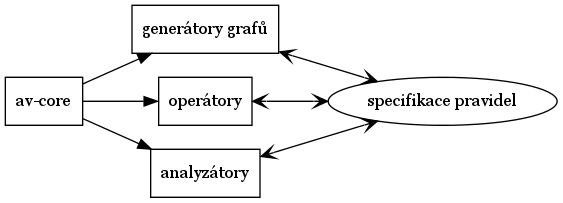
\includegraphics[width=0.8\textwidth]{./graphs/system_extensions.png}
  \caption{Body rozšíření systému.\label{design-system_extensions}}
\end{figure}

Vzhledem k~formalismu navrženému v~sekci \ref{design-graph_formalization} je nutné nejprve vhodným způsobem zpracovat vstup. K~tomu budou sloužit \emph{generátory grafů}. Jejich zodpovědností bude vygenerování určitého typu grafu z~AST analyzovaného programovacího jazyka.

Rozšíření typu \emph{operátor} představuje jeden konkrétní operátor (selektor nebo predikát), který je možné použít v~rámci \emph{souboru definic}. Každý operátor bude deklarovat své \emph{jméno}, \emph{počet} a \emph{typy operandů} a \emph{návratový typ}.

Protože ne všechny kontroly zdrojového kódu lze zapsat jako pravidla s~výsledkem \verb+true+ nebo \verb+false+, bude možné do systému vložit vlastní \emph{analýzu}, jejímž vstupem bude graf konkrétního typu. Nad tímto grafem bude analýza vyhodnocena a výstup ve vhodném vnitřním formátu bude předán vrácen jako výsledek.

Na základě provedené dekompozice definujeme seznam rozhraní, která budou muset být implementována poskytovateli služeb (service providers):

\begin{itemize}
\item \emph{GraphGeneratorIface} -- rozhraní poskytovatele generátoru grafu,
\item \emph{OperatorIface} -- rozhraní poskytovatele operátorů (selektorů a predikátů),
\item \emph{AnalysisIface} -- rozhraní poskytovatele analýzy (analytického modulu).
\end{itemize}

Každé z těchto rozšíření může být implementování více různými poskytovateli. Pouze je nutné zajistit, aby nekolidovaly názvy poskytovaných služeb (jména operátorů, typů generátorů grafů a názvy analýz).

Celá dekompozice provedená v~tomto stupni je zachycena v~diagramu komponent na obrázku \ref{design-modules}. Modul jádra nazveme \verb+av-core+.
\begin{figure}[h!]
  \centering
  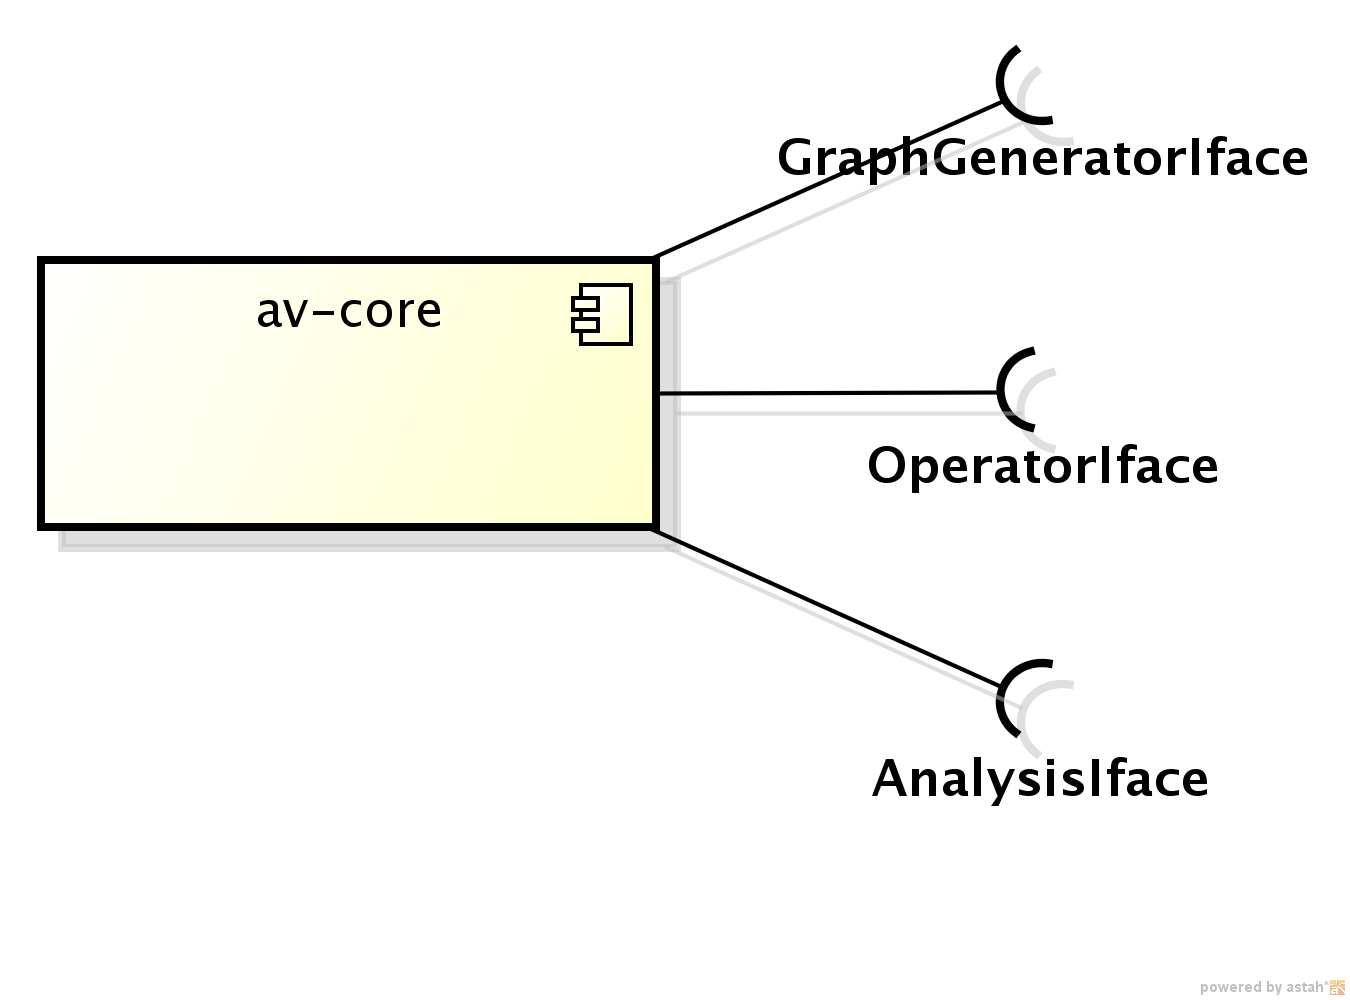
\includegraphics[width=0.5\textwidth]{./uml/archval_module_cmp.png}
  \caption{Dekompozice systému na jádro a rozšíření.\label{design-modules}}
\end{figure}
Jeho dekompozice bude provedena v~dalších sekcích. Ještě předtím se ale podíváme na důležité doménové objekty, které budou reprezentovat data předávaná mezi jednotlivými komponentami v~rámci systému.

\subsection{Doménové objekty}
\label{design-domain_objects}

Přehled doménových objektů podává tabulka \ref{design-domain_object_table}. Protože jsou tyto objekty součástí jádra a změna jejich rozhraní by nutně vedla k~úpravě ostatních komponent, navrhujeme tyto datové typy jako konkrétní třídy\footnote{U ostatních komponent předpokládáme, že budou implementovány třetími stranami. Je třeba pro ně třeba přesně definovat veřejná rozhraní SPI.}.

\begin{table}[h]
  \caption{Tabulka doménových objektů. \label{design-domain_object_table}}
  \begin{center}
    \begin{tabular}{| l | c | p{8cm} |}
      \hline
      \textbf{Název} & \textbf{Typ} & \textbf{Zodpovědnost} \\
      \hline
      \hline
      \emph{Graph} & class & graf reprezentující analyzované elementy \\ \hline
      \emph{Vertex} & class &  vrchol grafu \\ \hline
      \emph{Edge} & class & hrana grafu \\ \hline
      \emph{GraphModel} & class & množina grafů různých typů \\ \hline
      \hline
      \emph{ValidationModel} & class & model validace načtený ze vstupního \emph{souboru definic} \\ \hline
      \hline
      \emph{ValidationReport} & class &  objekt reprezentující výstup validace\\ \hline
    \end{tabular}
  \end{center}

\end{table}

\emph{Graph}, \emph{Vertex} a \emph{Edge} jsou elementárními datovými třídami představujícími vygenerovaný graf jeho vrcholy a hrany. V této práci navrhujeme tyto elementy jako třídy. Je možné tyto elementy zadefinovat též jako rozhraní. Tím  bychom získali možnost analyzovat zcela libovolné elementy (např. existující objektovou hierarchii). Důležitým elementem třída \emph{Graph} bude deklarace jejího typu, který si musí nést s sebou. Jednotlivé instance grafů různých typů seskupíme do jedné entity \emph{GraphModel}, kterou budeme dále v systému předávat jako celek. To bude množina\footnote{Každý typ grafu může být zahrnut právě jednou.} grafů různých typů.

Třída \emph{ValidationModel} představuje klíčovou komponentu nesoucí veškeré informace potřebné pro provedení validačního procesu. Bude se jednat o strom pravidel vygenerovaný na základě souboru specifikace pravidel, který bude mít schopnost se samostatně vyhodnotit na základě předané vstupní instance typ \emph{GraphModel}. Výsledkem vyhodnocení bude potom instance třídy \emph{ValidationReport}, která bude poskytovat informace o průběhu zpracování.

Navrhované třídy \emph{ValidationModel} a \emph{GraphModel} je možné vygenerovat a používat opakovaně (cache). To se může hodit v~případech, kdy chceme tentýž projekt (pro nějž jsme již jednou generovali graf) validovat pomocí jiné/upravené množiny pravidel nebo naopak pokud chceme použít jednu množinu pravidel pro validaci více projektů. Bylo by zbytečné opakovaně provádět náročné operace generování grafu nebo parsování souboru pravidel a navazování operátorů (popisováno dále).

Některé z těchto tříd rozebereme nyní detailněji:

\subsubsection{Třída ValidationModel}
Validační model (třída \emph{ValidationModel}) sestává z atomických pravidel a složených pravidel. Tato pravidla je nutné načíst z existujícího souboru specifikací a sestavit z nich strom vhodný pro vyhodnocení. Přesná definice vstupního souboru je popsána v příloze \ref{avd_grammar}. Zahrnuje specifikaci atomických pravidel, složených pravidel a příkazů, které umožní vybrat pouze konkrétní podmnožinu pravidel, která se mají ověřit a příkazů, které umožní provedení vybraných analýz.

To vše musí model vhodným způsobem reflektovat. Na základě vstupních elmenetů vygenerujeme AST (nejspíš pomocí vhodného nástroje), který následně převedeme na strom, který se bude skládat z jednotlivých operátorů a vstupních parametrů, který bude možné vyhodnotit nad existujícím instancí třídy \emph{GraphModel}.

Třídu dekomponujeme dále na třídy \emph{AtomicRule} a \emph{CompoundRule} (které budou mít společného předka \emph{Rule}, abychom mohli k těmto pravidlům při vyhodnocování přistupovat stejně. Tyto třídy budou dále obsahovat již konkrétní syntaktický strom uzlů, které budou mít metodu \emph{evaluate()}, která vždy zajistí vyhodnocení příslušeného uzlu a návrat výsledné hodnoty. Díky tomu bude vyhodnocení celého stromu pravidel (z hlediska uživatele modelu) triviální -- provedeme zavolání metody \emph{validate()} na kořenovém elementu komponenty \emph{ValidationModel}. Ta následně zavolá \emph{evaluate()} metody na svých potomcích a takto to bude probíhat až k listovým elementům.

Pro vybudování zmíněného stromového modelu vytvoříme samostanou komponentu \emph{ValidationModelGenerator}, jejíž rozhraní bude definováno dále.

\subsubsection{Třída ValidationReport}
\label{design-class_validation_report}
Výstupem validačního procesu bude objekt třídy \emph{ValidationReport}. Ačkoliv matematická pravidla popsaná výše mají jako výstup pouze logickou hodnotu. Je vhodné, aby bylo možné nějakým způsobem zjistit, v jaké fázi vyhodnocování došlo k nesplnění pravidla. Proto poskytneme právě datovou třídu \emph{ValidationReport}. Ta ponese nejen elementární výsledky pravidel, ale také mezivýsledky vyhodnocení jednotlivých uzlů syntaktického stromu popsaného dříve.

Strom výsledků dekomponujeme podobným způsobem, jakým jsme dekomponovali třídu \emph{ValidationModel}. Poskytneme třídy \emph{AtomicRuleResult} a \emph{ComopundRuleResult}. Tyto třídy opět oddědíme od společného předka, abychom je mohli uchovávat v rámci jednoho seznamu výsledků.

Kromě toho přidáme ještě třídu \emph{AnalysisResult}, která ponese informaci o konkrétní prováděné analýze. Pro třídu \emph{AnalysisResult} strom generovat nebudeme, protože neznáme přesný způsob práce konkrétního analytického modulu. Třída \emph{AnalysisResult} bude obsahovat seznam tvrzení o množinách vrcholů nebo hran. Každý záznam bude obsahovat vždy množinu vrcholů nebo hran a k ní řetězec, který bude obsahovat výrok, který platí. Způsob provádění analýz a zpracovávání výsledků je oblast, kterou je možné řešit samostatně v rámci dalších návazností této práce.

Generování objektů třídy \emph{ValidationReport} bude součástí průběhu zpracování validace. Metoda \emph{validate()} třídy \emph{ValidationModel} provede vytvoření objektu \emph{ValidationReport} a příslušných podobjektů (\emph{AtomicRuleResult}, atd.). Tyto objekty následně předá prostřednictvím \emph{evaluate()} metod do dalších vyhodnocovacích uzlů. Ty provedou totéž o úroveň níže. Každý uzel po provedení příslušné operace uloží do předaného objektu svou návratovou hodnotu. Díky tomu získáme strom obsahující data umožňující rekonstruovat průběh zpracování.



\subsection{Jádro systému}
Jádro systému samotné nebude poskytovat žádná konkrétní pravidla pro validaci ani žádné analýzy. Bude se jednat o platformu, která umožní přidávání nových komponent, které toto budou provádět na základě textového popisu pravidel. Součástí jádra budou komponenty nezbytné pro zpracování vstupního souboru definic do podoby vhodné k provedení (vytvoření modelů, navázání poskytovaných operátorů). Přehled navrhovaných komponent a rozhraní jádra uvádíme v tabulce v~tabulce \ref{design-archval_core_components}.

\begin{table}
  \caption{Tabulka komponent jádra systému. \label{design-archval_core_components}}
  \begin{center}
    \begin{tabular}{ | l | l | p{7.5cm} | }
      \hline
      \textbf{Název} & \textbf{Typ} & \textbf{Zodpovědnost} \\
      \hline
      \hline
      \emph{GraphModelGenerator} & class & zinicializuje jednotlivé moduly pro generování grafů a použije je pro vygenerování grafů (pokud jsou tyto grafy požadovány) \\ \hline
      \emph{GraphModelGeneratorIface} & interface & rozhraní předchozí komponenty \\ \hline
      \emph{ValidationModelGenerator} & class & generátor, který na základě validační specifikace vygeneruje instanci třídy \mbox{\emph{ValidationModel}} \\ \hline
      \emph{ValidationModelGeneratorIface} & interface & rozhraní předchozí komponenty \\ \hline
      \emph{ValidationTask} & class & hlavní proces validace \\ \hline
      \emph{ValidationTaskIface} & interface & rozhraní předchozí komponenty \\ \hline
      \hline
      \emph{ArchVal} & class & fasáda ArchVal systému -- bude poskytovat instance výše specifikovaných komponent \\ \hline
      \hline
      \emph{GraphGeneratorsRegisterIface} & interface & rozhraní registru existujících poskytovatelů generátorů grafu \\ \hline
      \emph{OperatorsRegisterIface} & interface & rozhraní registru existujících poskytovatelů operátorů \\ \hline
      \emph{AnalysesRegisterIface} & interface & rozhraní registru poskytovatelů komponent analýzy \\ \hline
    \end{tabular}
  \end{center}

\end{table}

Vztahy mezi jednotlivými komponentami jádra systému jsou znázorněny na obrázku \ref{design-archval_core}. Komponenta \emph{ArchVal} bude zastřešovat přístup k funkcionalitám jádra. Díky tomu budeme moci komponenty \emph{GraphModelGenerator}, \emph{ValidationModelGenerator} a \emph{ValidationTask} skrýt za vhodná rozhraní a v případě potřeby je reimplementovat. Všimněme si komponent \emph{GraphGeneratorsRegisterIface}, \emph{OperatorsRegisterIface} a \emph{AnalysesRegisterIface}. Ty představují rozhraní samostatných komponent, které nám budou schopny poskytnout poskytovatele implementace existujících rozšíření (generátory grafů, operátory a analýzy). Díky této abstrakci bude jádro systému možné zakomponovat do jakékoliv platformy bez nutnosti uvažovat mechanismy pro registraci poskytovatelů služeb\footnote{Jak uvidíme dále v části \emph{Implementace}, registrace poskytovatelů je vždy nějakým způsobem nutná a různé platformy ji podporují různým způsobem. Zmiňme \emph{Lookup} na platformě NetBeans nebo nově přidanou vlastnost jazyka Java verze 6 \emph{ServiceLoader}.}.

\begin{figure}[h!]
  \centering
  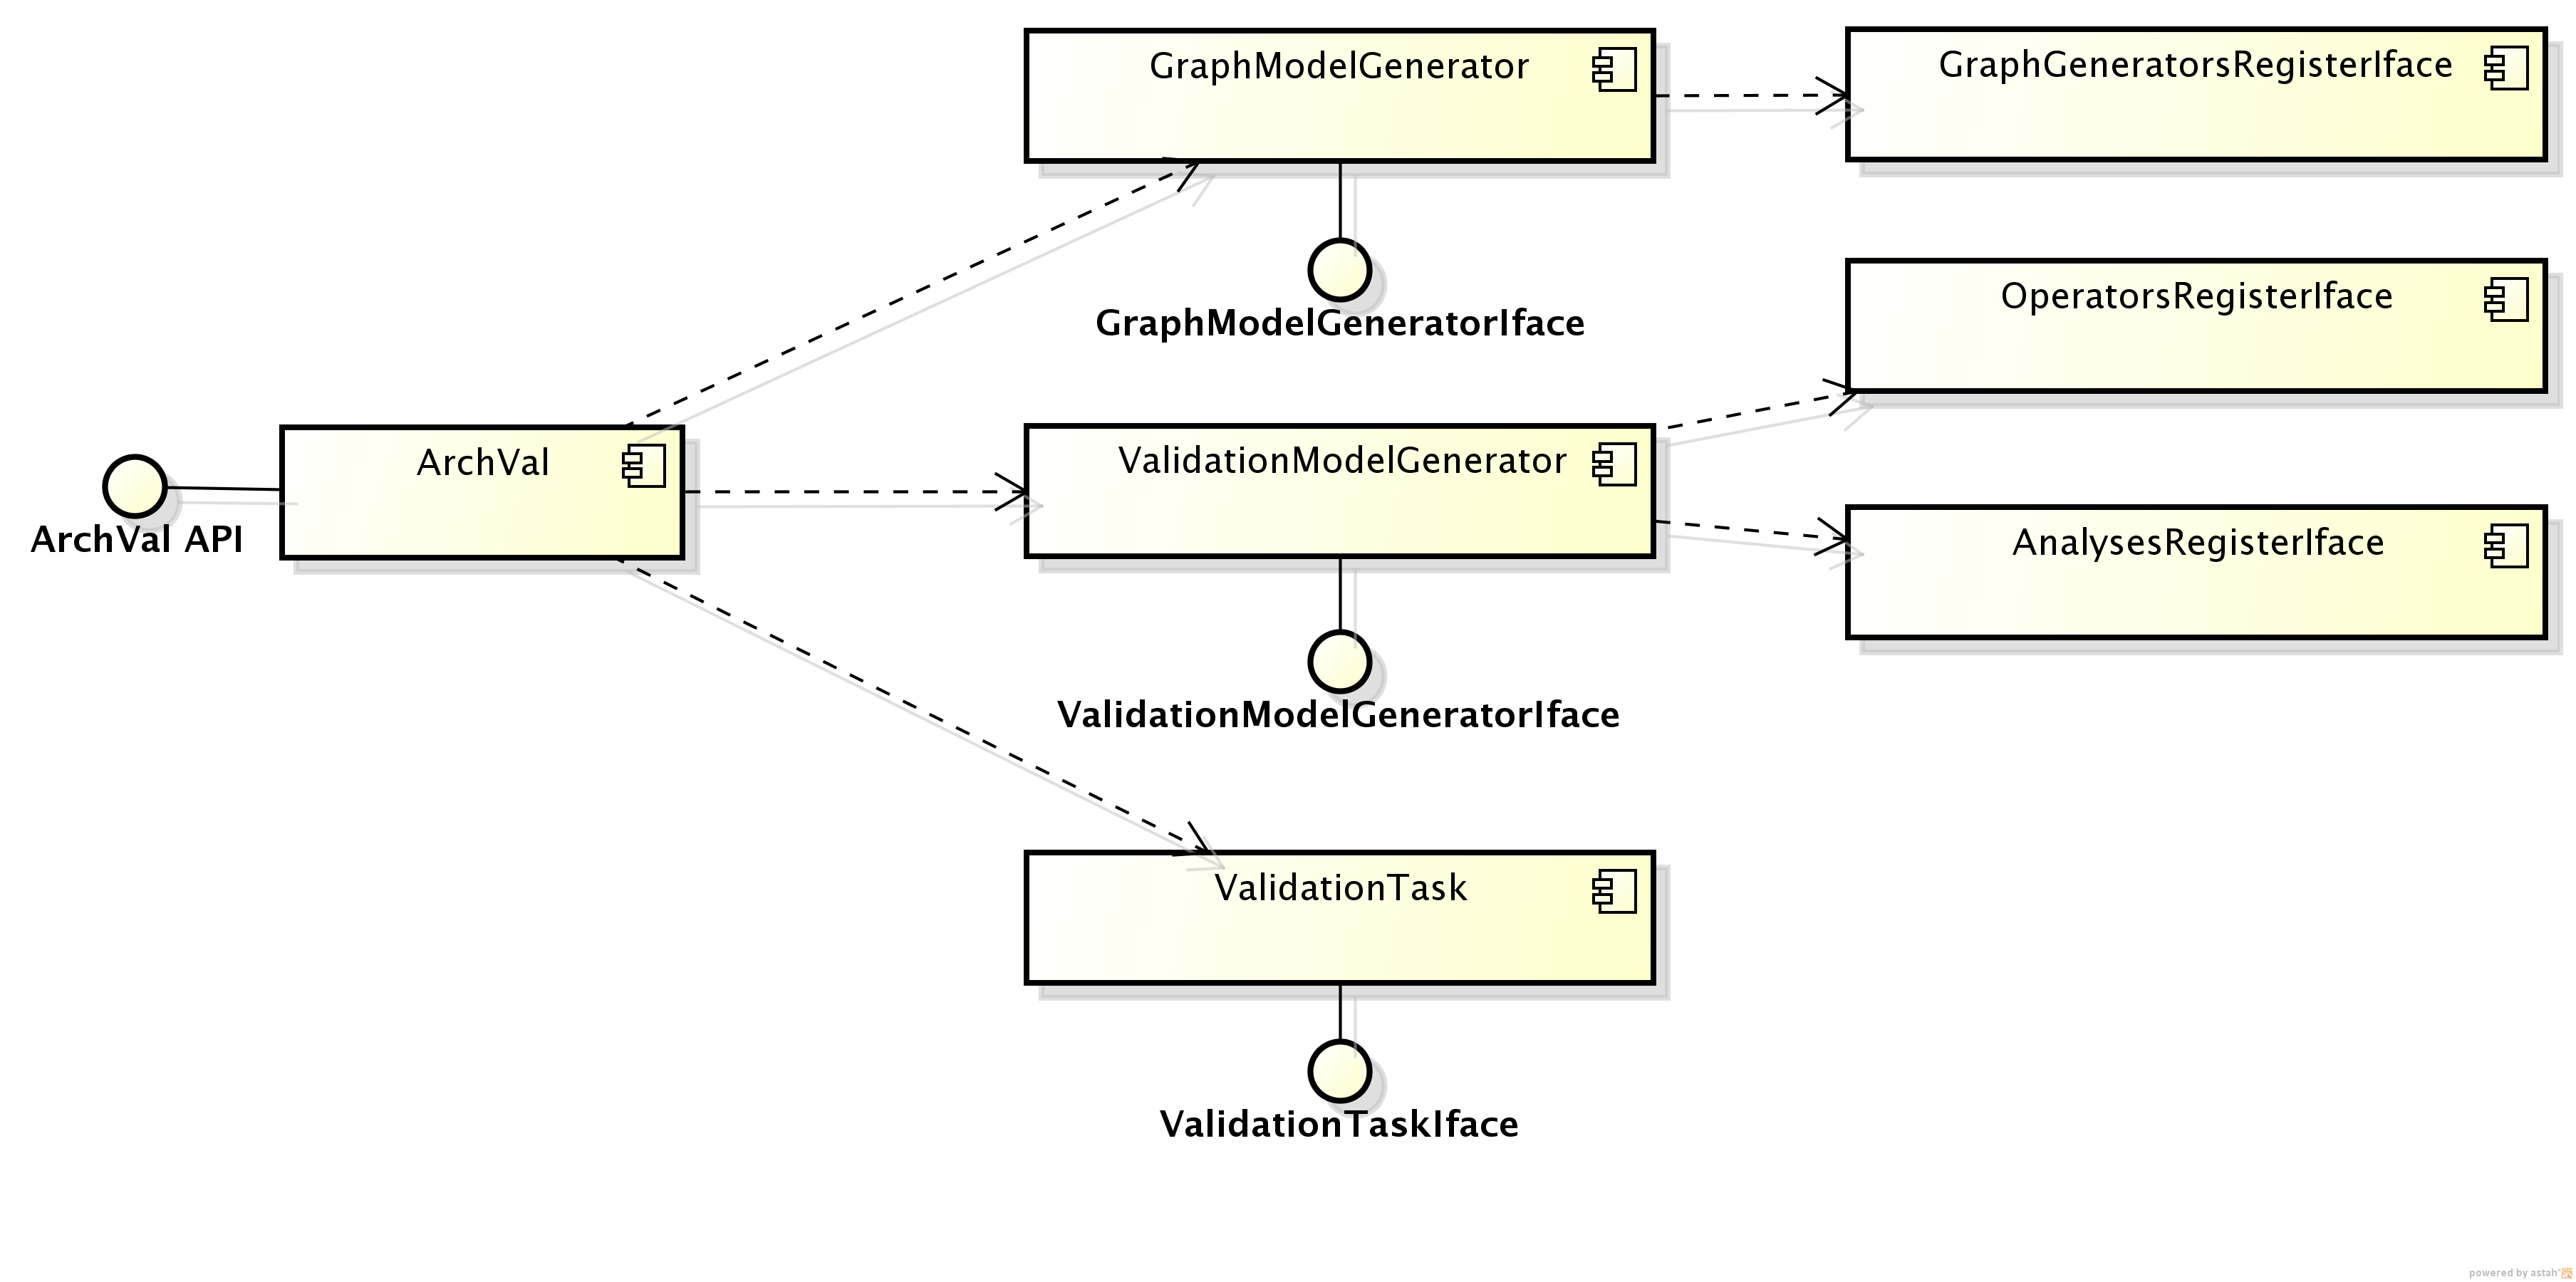
\includegraphics[width=1.0\textwidth]{./uml/archval_core_cmp.png}
  \caption{Komponenty jádra systému ArchVal.\label{design-archval_core}}
\end{figure}

\subsubsection{Komponenta GraphModelGenerator}
Komponenta \emph{GraphModelGenerator} bude mít na zodpovědnosti vygenerování všech grafů potřebných pro provedení analýzy. Abychom mohli časem komponentu reimplementovat, skryjeme její implementaci za rozraní \emph{GraphModelGeneratorIface}. To bude vystupovat v kontaktu s \uv{vnějšími} entitami jádra (u klientského uživatele knihovny jádra ArchVal). Jak je patrné již z obrázku \ref{design-archval_core}, tato komponenta má závislost na rozhraní \emph{GraphGeneratorsRegisterIface}. Samotná komponenta \emph{GraphModelGenerator} vlastně žádné grafy generovat přímo nebude. Bude k tomuto úkolu využívat některé z dostupných generátorů grafů dostupných prostřednictvím registru.

\begin{figure}[h!]
  \centering
  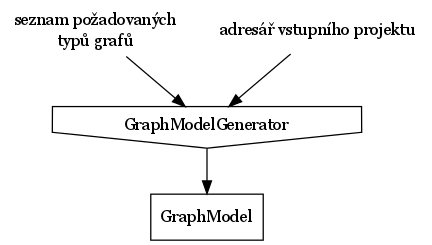
\includegraphics[width=0.6\textwidth]{./graphs/graph_generator_io_graph.png}
  \caption{Znázornění vstupů a výstupů komponenty typu \emph{GraphModelGenerator}.\label{design-graph_generator_io}}
\end{figure}

Vstupy a výstupy komponenty jsou znázorněny na obrázku \ref{design-graph_generator_io}. U vstupů se jedná o adresář obsahující vstupní Java soubory analyzovaného projektu a seznam identifikátorů typů grafů, které chceme vygenerovat. Výstup je potom představován instancí třídy \emph{GraphModel}. Je možné, že komponenta  \emph{GraphModelGenerator} nebude mít k dispozici potřebné generátory grafů. V tom případě vyhodí výjimku.

\paragraph{Rozhraní}
Rozhraní této komponenty bude představováno jedinou metodou:
\begin{itemize}
\item \begin{verbatim}generateModel(Set<String> requiredGraphTypes,
              File projectDirectory) : GraphModel\end{verbatim}
\end{itemize}

Poznamenejme, že v rozhraních budeme uvádět datové typy jazyka Java, což není z~hlediská návrhu zcela správné, nicméně pro potřeby této práce to bude postačující.

\subsubsection{Komponenta ValidationModelGenerator}
Druhou významnou vstupní komponentou je vedle genrátoru modelu grafu komponenta \emph{ValidationModelGenerator}, která bude sloužit k vygenerování instance dříve popsané doménové třídy \emph{ValidationModel}. Tato komponenta má na zodpovědnosti zpracování vstupního souboru, který jí bude ve vhodné podobě předán a vytvoření stromové struktury třídy \emph{ValidationModel}, která bude umět provést vyhodnocení pravidel specifikovaných vstupním souborem, vyhodnocení analýz a vygenerování výsledného objektu třídy \emph{ValidationReport}. Podobně jako předchozí komponentu i tuto zpřístupníme jako rozhraní, v tomto případě rozhraní \emph{ValidationModelGeneratorIface}.

\begin{figure}[h!]
  \centering
  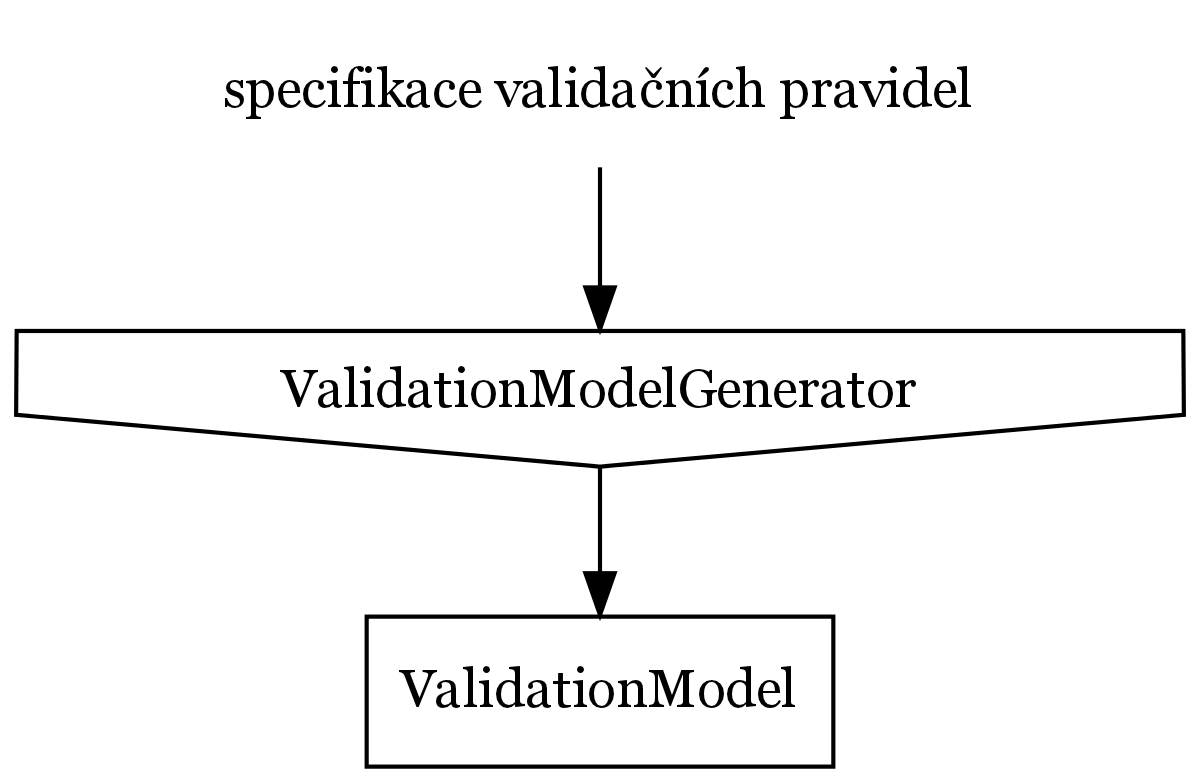
\includegraphics[width=0.55\textwidth]{./graphs/validation_model_generator_io_graph.png}
  \caption{Znázornění vstupů a výstupů komponenty \emph{ValidationModelGenerator}.\label{design-validation_model_generator_io}}
\end{figure}

Znázornění vstupů a výstupů komponenty \emph{ValidationModelGenerator} je na obrázku \ref{design-validation_model_generator_io}. Vstupem je množina pravidel zapsaná ve formátu AVD. Ta může být zadána buď jako vstupní \emph{stream} nebo řetězec\footnote{Tato možnost zde byla přidána z ohledem na možnost přímé integrace, kdy by uživatel mohl zadávat pravidla do nějakého textového vstupu aplikace a tato pravidla byla rovnou použita pro validaci projektu.}. Výstupem kpomonenty je instance třídy \emph{ValidationModel}.

\paragraph{Rozhraní} Rozhraní komponenty je představováno metodami:

\begin{itemize}
\item \verb-constructValidationModel(InputStream is) : ValidationModelIface-
\item \verb-constructValidationModel(String string) : ValidationModelIface-
\end{itemize}

\subsubsection{Komponenta ValidationTask}
\label{design-component_validation_task}
Centrální komponentou umožňující spuštění validačního procesu bude \emph{ValidationTask} (implementace skrytá za \emph{ValidationTaskIface}). Tato komponenta bude mít na starosti provedení validačního procesu pomocí komponent \emph{ValidationModel} a \emph{GraphModel}. Implementace bude poměrně triviální, vzhledem k faktu, že veškerá logika potřebná k provedení validace bude zapouzdřena již v komponentě \emph{ValidationModel}. Komponenta \emph{ValidationTask} tak bude mít na starosti zajištění bezpečného spouštění procesu validace a to jak synchronním způsobem tak asynchronně (v samostaném vlákně).

\paragraph{Rozhraní} Rozhraní komponenty \emph{ValidationTask} bude představováno následujícími metodami:
\begin{itemize}
\item \verb-runSynchronous() : void- -- synchronní spuštění validace
\item \verb-runAsynchronous() : void- -- běh validace v samostatném vlákně
\item \begin{verbatim}registerValidationCompletedListener(
    ValidationCompletedListener validationCompletedListener
) : void\end{verbatim} -- registrace listeneru, který bude notifikován o doběhnutí procesu validace
\item \verb-getReport() : ValidationReport- -- vrátí instanci třídy \emph{ValidationReport}
\end{itemize}

Výsledný objekt \emph{ValidationReport} si volající může zpracovat libovolným způsobem. Například je možné ji reprezentovat ve vhodné swing komponentě (JTree).

\subsubsection{Komponenta ArchVal (fasáda)}
Předchozí komponenty zapouzdříme pomocí návrhového vzoru fasáda, za nímž skryjeme detaily implmentace. Poskytneme tak službu pro získání hotových komponent pro generování modelů. Navíc můžeme tímto způsobem zajistit, aby pro každou instanci třídy \emph{ArchVal} byly k dispozici třídy \emph{ValidationModelGenerator} a \emph{GraphModelGenerator} pouze v jedné instanci.

\paragraph{Rozhraní} Rozhraní je představováno následujícími metodami:
\begin{itemize}
\item \begin{verbatim}ArchVal(
    GraphGeneratorsRegisterIface graphGeneratorsRegister,
    OperatorsRegisterIface operatorsRegister,
    AnalysesRegisterIface analysesRegister) : ArchVal\end{verbatim}
\item \verb-GraphModelGeneratorIface getGraphModelGenerator()-
\item \verb-ValidationModelGeneratorIface getValidationModelGenerator()-
\item \begin{verbatim}ValidationTaskIface createValidationTask(
    GraphModel graphModel,
    ValidationModelIface validationModel) : GraphModel\end{verbatim}
\end{itemize}

Metoda \verb-createValidationTask()- představuje tovární metodu, která vrátí pokaždé nový objekt \emph{ValidationTask}\footnote{Vzhledem k možnosti asynchronního provolávání metod třídy \emph{ValidationTask} je požadováno, aby každá instance \emph{ValidationTask} byla použita nejvýše jednou.}.

\subsubsection{Rozhraní registrů poskytovatelů implementací}

Jak bylo zmíněno již v sekci \ref{desing-global_system_structure}, rozšíření budou získávána pomocí rozhraní \emph{GraphGeneratorsRegisterIface}, \emph{OperatorsRegisterIface} a \emph{AnalysesRegisterIface}. Zde uveďme operace, které požadujeme od těchto rozhraní:

\paragraph{Rozhraní GraphGeneratorsRegisterIface} Od registru generátorů grafů budeme požadovat, aby byl schopen vrátit seznam všech dostupných typů generátorů a dále konkrétní generátor na základě typu.
\begin{itemize}
\item \verb-getAvaliableGeneratorTypes() : Set<String>-
\item \verb-getGraphGeneratorByType(String type) : GraphGeneratorIface-
\end{itemize}

\paragraph{Rozhraní OperatorsRegisterIface}
Zde požadujeme pouze zisk existujícího operátoru na základě jména. Pokud by bylo časem nutné podpořit editaci AVD souborů, zcela jistě by bylo potřeba získat i úplný seznam operátorů, případně implementovat vyhledávání i podle jiných kritérií (např. návratová hodnota).

\begin{itemize}
\item getOperatorByName(String name) : OperatorIface
\end{itemize}

\paragraph{Rozhraní AnalysesRegisterIface} Zpravidla budeme potřebovat pouze metodu na zisk existujícího analytického modulu na základě jeho názvu. Přesto poskytujeme i metodu, která umožní získat seznam všech existujících analytických modulů.

\begin{itemize}
\item getAnalysesList() : List<AnalysisIface>
\item getAnalysisByName(String name) : AnalysisIface
\end{itemize}

\subsection{Rozhraní rozšíření systému}

Nyní se podívejme na vlastní rozhraní, která musí být implementovaná poskytovali služeb poskytovaných prostřednictvím výše zmíněných registrů. Jedná se o rozhraní \emph{GraphGeneratorIface}, \emph{OperatorIface} a \emph{AnalysisIface}.

\subsubsection{Rozhraní GraphGeneratorIface}
Úkolem implementátora generátoru grafu je zaimplementovat rozhraní \emph{GraphGeneratorIface}. Toto rozhraní bude definovat následující operace:
\begin{itemize}
\item \verb-getGraphType() : String- -- typ grafu, který produkuje tento generátor grafu
\item \verb-getGraph(File projectDirectory) : Graph- -- metoda, která provede vlastní vygenerování grafu
\end{itemize}

Vstupem pro metodu pro generování grafu je specifikace adresáře, který obsahuje projekt, z něhož má být vygenerován grafový model. Každý generátor musí vracet id typu grafu, který generuje. Systém odmítne spustit validaci, pokud bude obsahovat více poskytovatelů generátoru grafu, kteří poskytují generování grafu stejného typu.

\subsubsection{Rozhraní OperatorIface}
Soubory specifikací pravidel mohou obsahovat volání predikátů a selektorů. Všechny tyto operátory musí implementovat rozhraní \emph{OperatorIface}. Rozhraní obsahuje všechny potřebné metody, které jsou nezbytné pro vykonání operátoru. Jedná se o jméno operátoru (odpovídá jménu uvedenému v AVD souboru), počet a typ operandů a jeho návratovou hodnotu.

\begin{itemize}
\item \verb-getName() : String- -- název operátoru
\item \verb-getOperandsCount() : int- -- počet operandů
\item \verb-getOperandType(int index) : DataType- -- typy operátoru na pozici udávané indexem
\item \verb-getReturnType() : DataType- -- návratový typ
\item \verb-execute(Graph graph, List<Object> operands) : Object- -- metoda umožňující provedení operátoru se specifikovanými parametry
\end{itemize}

Datové typy používané u opratorů odpovídají datovým typům zmiňovaným dříve v podsekci \ref{design-rules_formalization} (množina vrcholů, množina hran, atd.). V Jazyce java můžeme identifikátory těchto typů realizovat jako výčtový datový typ \verb-enum-.

\subsubsection{Rozhraní AnalysisIface}
Rozhraní \emph{AnalysisIface} reprezentuje jednu konkrétní analýzu, kterou je možné provést nad grafem konkrétního typu. To, nad jakým grafem lze analýzu spustit deklaruje analýza prostřednictvím metody -getRequiredGraphType() : String-. Podobně jako ostatní komponenty rozšíření musí i analýza specifikovat své jméno.

\begin{itemize}
\item \verb-getAnalysisName() : String-
\item \verb-getRequiredGraphType() : String-
\item \verb-evaluate(Graph graph) : AnalysisResult-
\end{itemize}

Výsledkem provedené analýzy je instance třídy \emph{AnalysisResult} zmiňovaná dříve v podsekci \ref{design-class_validation_report}.

\subsection{Základní průběh validačního procesu}
Hlavním vstupním bodem pro provedení validačního procesu je komponenta \emph{ValidationTask} popsaná dříve v podsekci \ref{design-component_validation_task}.

Systém nejprve vygeneruje validační model pomocí komponenty \emph{ValidationModelGenerator}. Na základě vygenerovaného modelu je potom možné získat seznam požadovaných typů grafů, které jsou nezbytné pro provedení validace a analýzy.

Seznam požadovaných typů grafů je následně předán komponěntě \emph{GraphModelGenerator}, která vygeneruje instanci třídy \emph{GraphModel} (resp. \emph{GraphModelIface}).

\emph{ValidationTask} následně předá získanou instanci \emph{GraphModelIface} validačnímu modelu (pomocí metody \emph{validate()}.

Po provedení validace (ať už synchronním nebo asynchronním\footnote{V případě asynchronního způsobu je nutné si zaregistrovat listener, který bude notifikován o doběhnutí vlákna validace.} způsobem) lze získat výsledky validace pomocí metody \emph{getReport()} třídy \emph{ValidationTask} výslednou instanci třídy \emph{ValidationReport}, kterou je možné vhodným způsobem prezentovat uživateli nebo jinak využít.

\section{Návrh vstupního rozhraní (zadávání pravidel)}
V sekci \ref{design-rules_formalization} byl stanoven způsob specifikace validačních pravidel. To, jakým způsobem budeme pravidla do systému zadávat, závisí do značné míry na případech užití realizovaného nástroje. Jednou možností je přímá specifikace pravidel prostřednictvím nějakého textového pole v grafickém uživatelském prostředí, jinou možností je zadání cesty k existujícímu AVD souboru.

Pro navrhovaný systém použijeme kombinovanou možnost. Umožníme přímou editaci editaci AVD souboru v prostředí nástroje a bude-li to možné, poskytneme další formy podpory editace (zvýrazňování syntaxe). Při vlastním procesu validace však budeme načítat již pravidla z vybraného existujícího souboru.

\section{Návrh výstupního rozhraní (provádění validace)}

Vzhledem k navržené architektuře je definice způsobu výstupu ponechána jako oblast, kterou lze řešit poměrně nezávisle. Po provedení validační úlohy (třída \emph{ValidationTask} je možné získat výstup třídy \emph{ValiationReport}. Tento výstup je následně možné zpracovat libovolným způsobem.

Uveďme možnosti dalšího zpracování výstupního reportu:

\begin{itemize}
\item export v některém existujícím standardním formátu - html, pdf, tex, ad.,
\item export prostého textového výstupu ve vlastním formátu,
\item textový výstup v okně aplikace,
\item reprezentace výstupu vhodnou swing komponentou (např. JTree komponenta).
\end{itemize}

Pro potřeby této práce postačí jednoduchý textový výstup, který pro realizovaná pravidla vypíše pouze zda pro daný vstup platí či nikoliv. Zpětné procházení stromu a vyhledávání příčin porušení konkrétního pravidla je ponecháno pro budoucí zpracování\footnote{Nicméně model byl záměrně navržen tak, aby toto podporoval -- výsledkem validace bude strom výsledků pro jednotlivé uzly pravidla, jak bylo popsáno dříve v podsekci \ref{design-class_validation_report}.}.

\section{Návrh způsobu integrace do různých typů prostředí}
Aplikační rozhraní systému \emph{ArchVal} je od začátku navrhováno tak, aby bylo možné jej zaintegrovat do libovolné aplikace. Díky nezávislosti na konkrétním způsobu poskytování implementátorů služeb je možné integrovat výsledný vyhodnocovací systém například do:

\paragraph{CLI programy} V~případě integrace prostředí ArchVal do samostatných skriptů a programů pro příkazovou řádku by bylo nutné zaimplementovat nějaký způsob registrace poskytovatelů služeb. To ale mohou být prosté texové soubory s~výčtem tříd, které se mají načíst. Případně mohou být seznamy operátorů definovány přímo v konkrétní implementaci registru operátoru, apod. U řádkových rozhraní je komplikovaná podpora editace AVD souborů.

\paragraph{GUI prostředí} Systém může být integrován do existujících prostředí IDE. V této práci navrhujeme a realizujeme integraci systému do prostředí NetBeans IDE. Současně využíváme výhod existujícího parseru zdrojových kódů jazyka Java. Podobně bychom mohli využít platformu \emph{Eclipse} nebo jiné prostředí. Na platormně NetBeans je možné implementovat registry poskytovatlů služeb velmi pohodlně pomocí tzv. \emph{Lookup API}, které je schopné poskytnout existující implementace konkrétního rozhraní\footnote{Stačí zaregistrovat poskytovatele služby v souboru \emph{META-INF/services}.}.

\section{Návrh technologií pro implementaci}
Pro implementaci systému použijeme jazyk \emph{Java 1.6} a platformu \emph{NetBeans} verze \emph{9.6.1}\footnote{V době realizace práce majoritní verze.}.  Pro zpracovávání zdrojových kódů využijeme prostředků poskytovaných touto platformou (\emph{Java Source API}).

Abychom mohli předpokládat pevnou strukturu vstupních projektů, omezíme možné vstupní projekty na standardní \emph{Maven Java projekty}.
